\section{System Architecture} \label{sec:sysarc}


The LSST control system is based on a reactive data-driven actor-based architecture that uses a multi cast Data Distribution Service (DDS) messaging protocol middleware. A high level view of this architecture is given in \figref{fig:arc}, where each box corresponds to a component of the system (not all components are displayed here).

The LSST System Architecture is comprised mainly of;
%
\begin{itemize}
\item The Service Abstraction Layer (SAL\footnote{\url{https://docushare.lsstcorp.org/docushare/dsweb/Get/Document-21527/}}) communication middleware. Based on the DDS protocol, it provides interfaces for all the project adopted programming languages (LabView, C++, Java and Python).
\item Engineering and Facility Database (EFD).
\item SAL-aware reactive components, a.k.a Commandable SAL Components (CSCs).
\item LSST Operators Visualization Environment (LOVE).
% \item Python SalObj\footnote{\url{https://github.com/lsst-ts/ts_salobj}} library.
%\item LabView component template.
% \item Script Queue  \footnote{\url{https://github.com/lsst-ts/ts_scriptqueue}}
\end{itemize}

\begin{figure}
\begin{center}
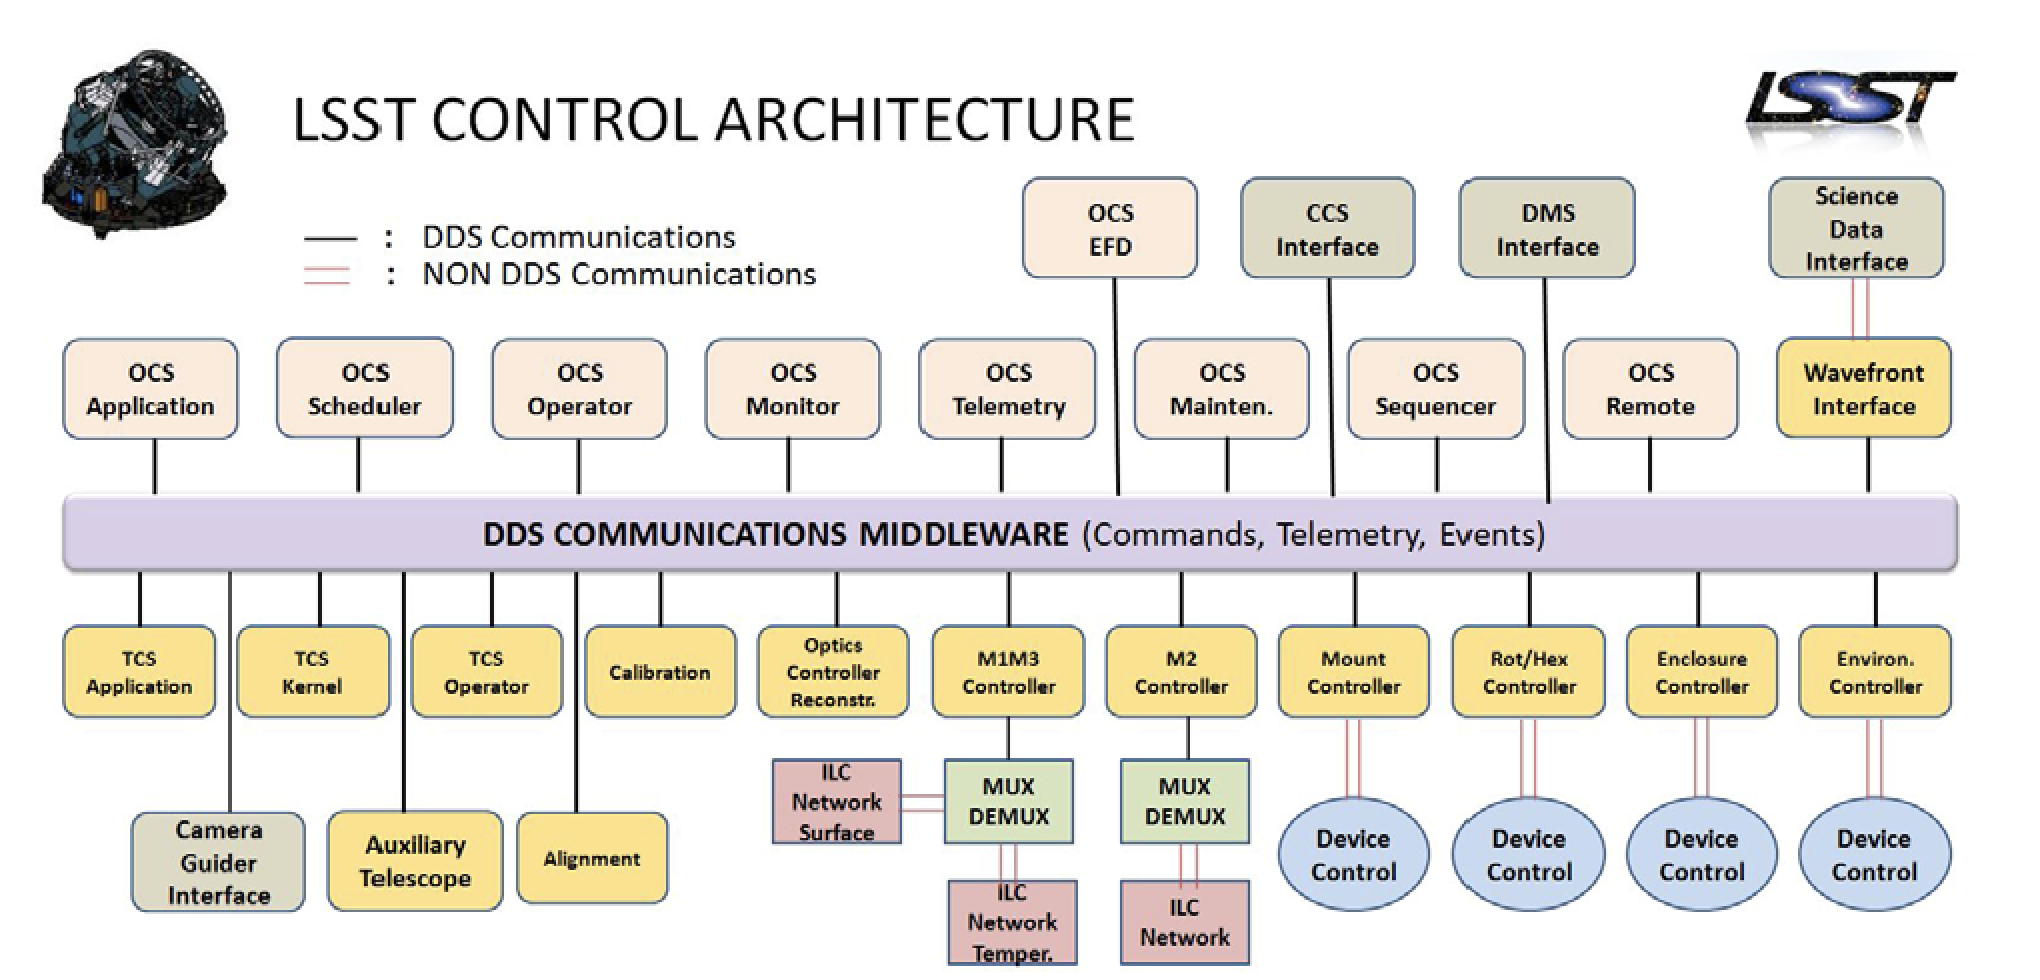
\includegraphics[width=0.8\textwidth]{arc}
\caption{High Level Architecture Diagram. (To be replaced...)\label{fig:arc}}
\end{center}
\end{figure}

The SAL middleware is the backbone of the LSST system architecture. It implements three distinct types of messages; Commands, Events and Telemetry, with distinct purposes. Commands are sent to a specific component, which must acknowledge its receipt and perform some action. In general, the receiving component will be the only entity listening for the commands it accepts\footnote{But note that the EFD, for instance, will also be listening for commands, though it will not acknowledges them.}. Events and Telemetry are messages broadcast by components to the middleware and are available to any entity on the system to receive. The distinction between Events and Telemetry is that the former with a higher Quality of Service (QoS) by the message passing system. It is also a general convention that Events have an asynchronous behavior, whereas Telemetry typically stream at a particular frequency.

The EFD is responsible for capturing all SAL messages broadcasts to the middleware (including Commands, Events and Telemetry) and storing that information into a database.

CSCs are the main actors of the LSST system architecture. They are responsible for managing the incoming traffic of data and take appropriate actions, controlling hardware (e.g. M1M3, M2, Mount Controller, etc in Fig.~\ref{fig:arc}), software (e.g. Optics Controller Reconstructor, DMCS Interface, etc in Fig.~\ref{fig:arc}) or even other CSCs (e.g. ScriptQueue, TCS, ATCS, OCS, etc in Fig.~\ref{fig:arc} ).

LOVE is responsible for capturing SAL messages and displaying them in a useful way for general users, providing some basic interface to query and analyze data from the EFD, an interface to issue pre-defined commands to a set of components and user interaction with the ScriptQueue (see Sect.~\ref{sect:scriptq}).

The SAL processes XML based definitions of the Commands, Events, and Telemetry for each CSC. Using this information, it creates runtime objects which support the messaging required. These take the form of shared libraries (C++, Python, LabVIEW) or Jar archives (Java) which implement consistent namespaces and API's. Other assets such as Simulated data, Sql table definitions, and web based documentation, may also be generated. On top of these low level APIs, developers have access to two higher-level set of frameworks; Python SalObj\footnote{\url{https://github.com/lsst-ts/ts_salobj}} library and the LabVIEW component template. No higher level framework is supported for implementations in Java or C++.

% a Python library (e.g. SalObj) or the LabView component template. There is no higher level support for implementation in Java or C++.

% Each component of the system is and independent actor that reacts to data published to the middleware.

%\begin{itemize}
%\item Infrastructure and Middleware :
%\item The Scheduler \footnote{\url{https://github.com/lsst-ts/ts_scheduler}}
%\item Potentially an Auxiliary and Main Telescope Control System (ATCS and TCS)\footnote {The precise nature and need for these is unclear now so they have lower priority.}
%\item Controllable SAL Components (CSCs) - every device and some pseudo devices, including the scheduler, are CSCs. Some are coordinating other CSCs, the full hierarchy is shown for AuxTel in \figref{fig:atcscs} and the Main Telescope in \figref{fig:mtcscs}
%\end{itemize}

Overall, the system architecture can be divided into three main namespaces; Observatory, Main Telescope (MT) and Auxiliary Telescope (AT). The Observatory is the highest level and encapsulates both the Main Telescope, Auxiliary Telescope and global components such as the weather station, DIMM, etc. The complete set of components that belong to each of these namespaces can be seen in Figs.~\ref{fig:ocs}, ~\ref{fig:atcscs} and \ref{fig:mtcscs}.

\begin{figure}
\begin{center}
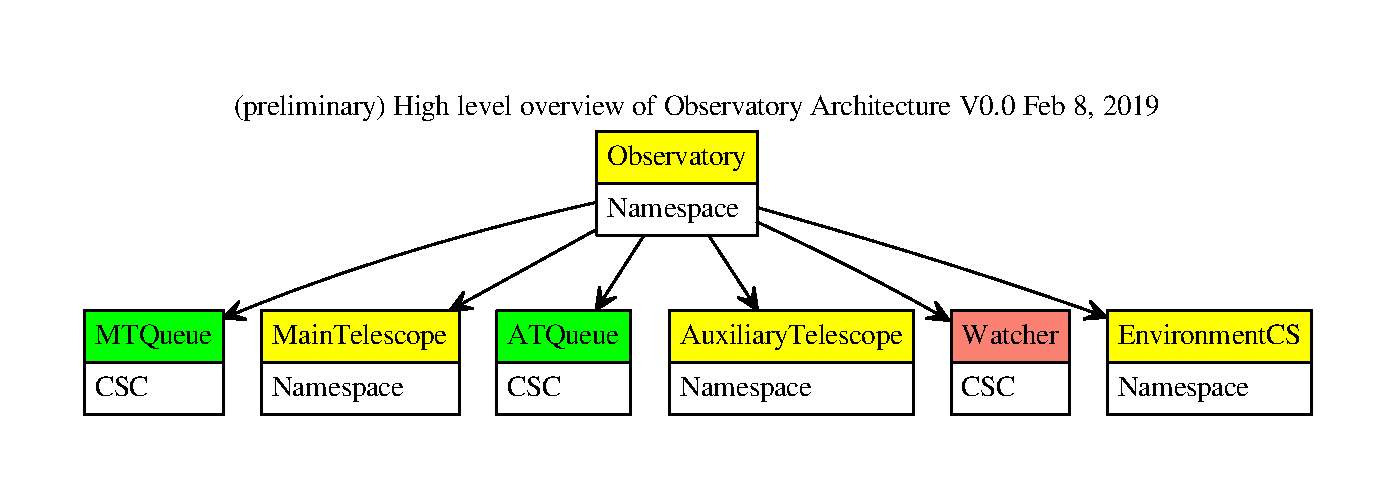
\includegraphics[width=0.9\textwidth]{Obs}
\caption{Hi level observatory architecture with namespaces and observatory-wide CSCs. (preliminary)\label{fig:ocs}}
\end{center}
\end{figure}

\begin{figure}
\begin{center}
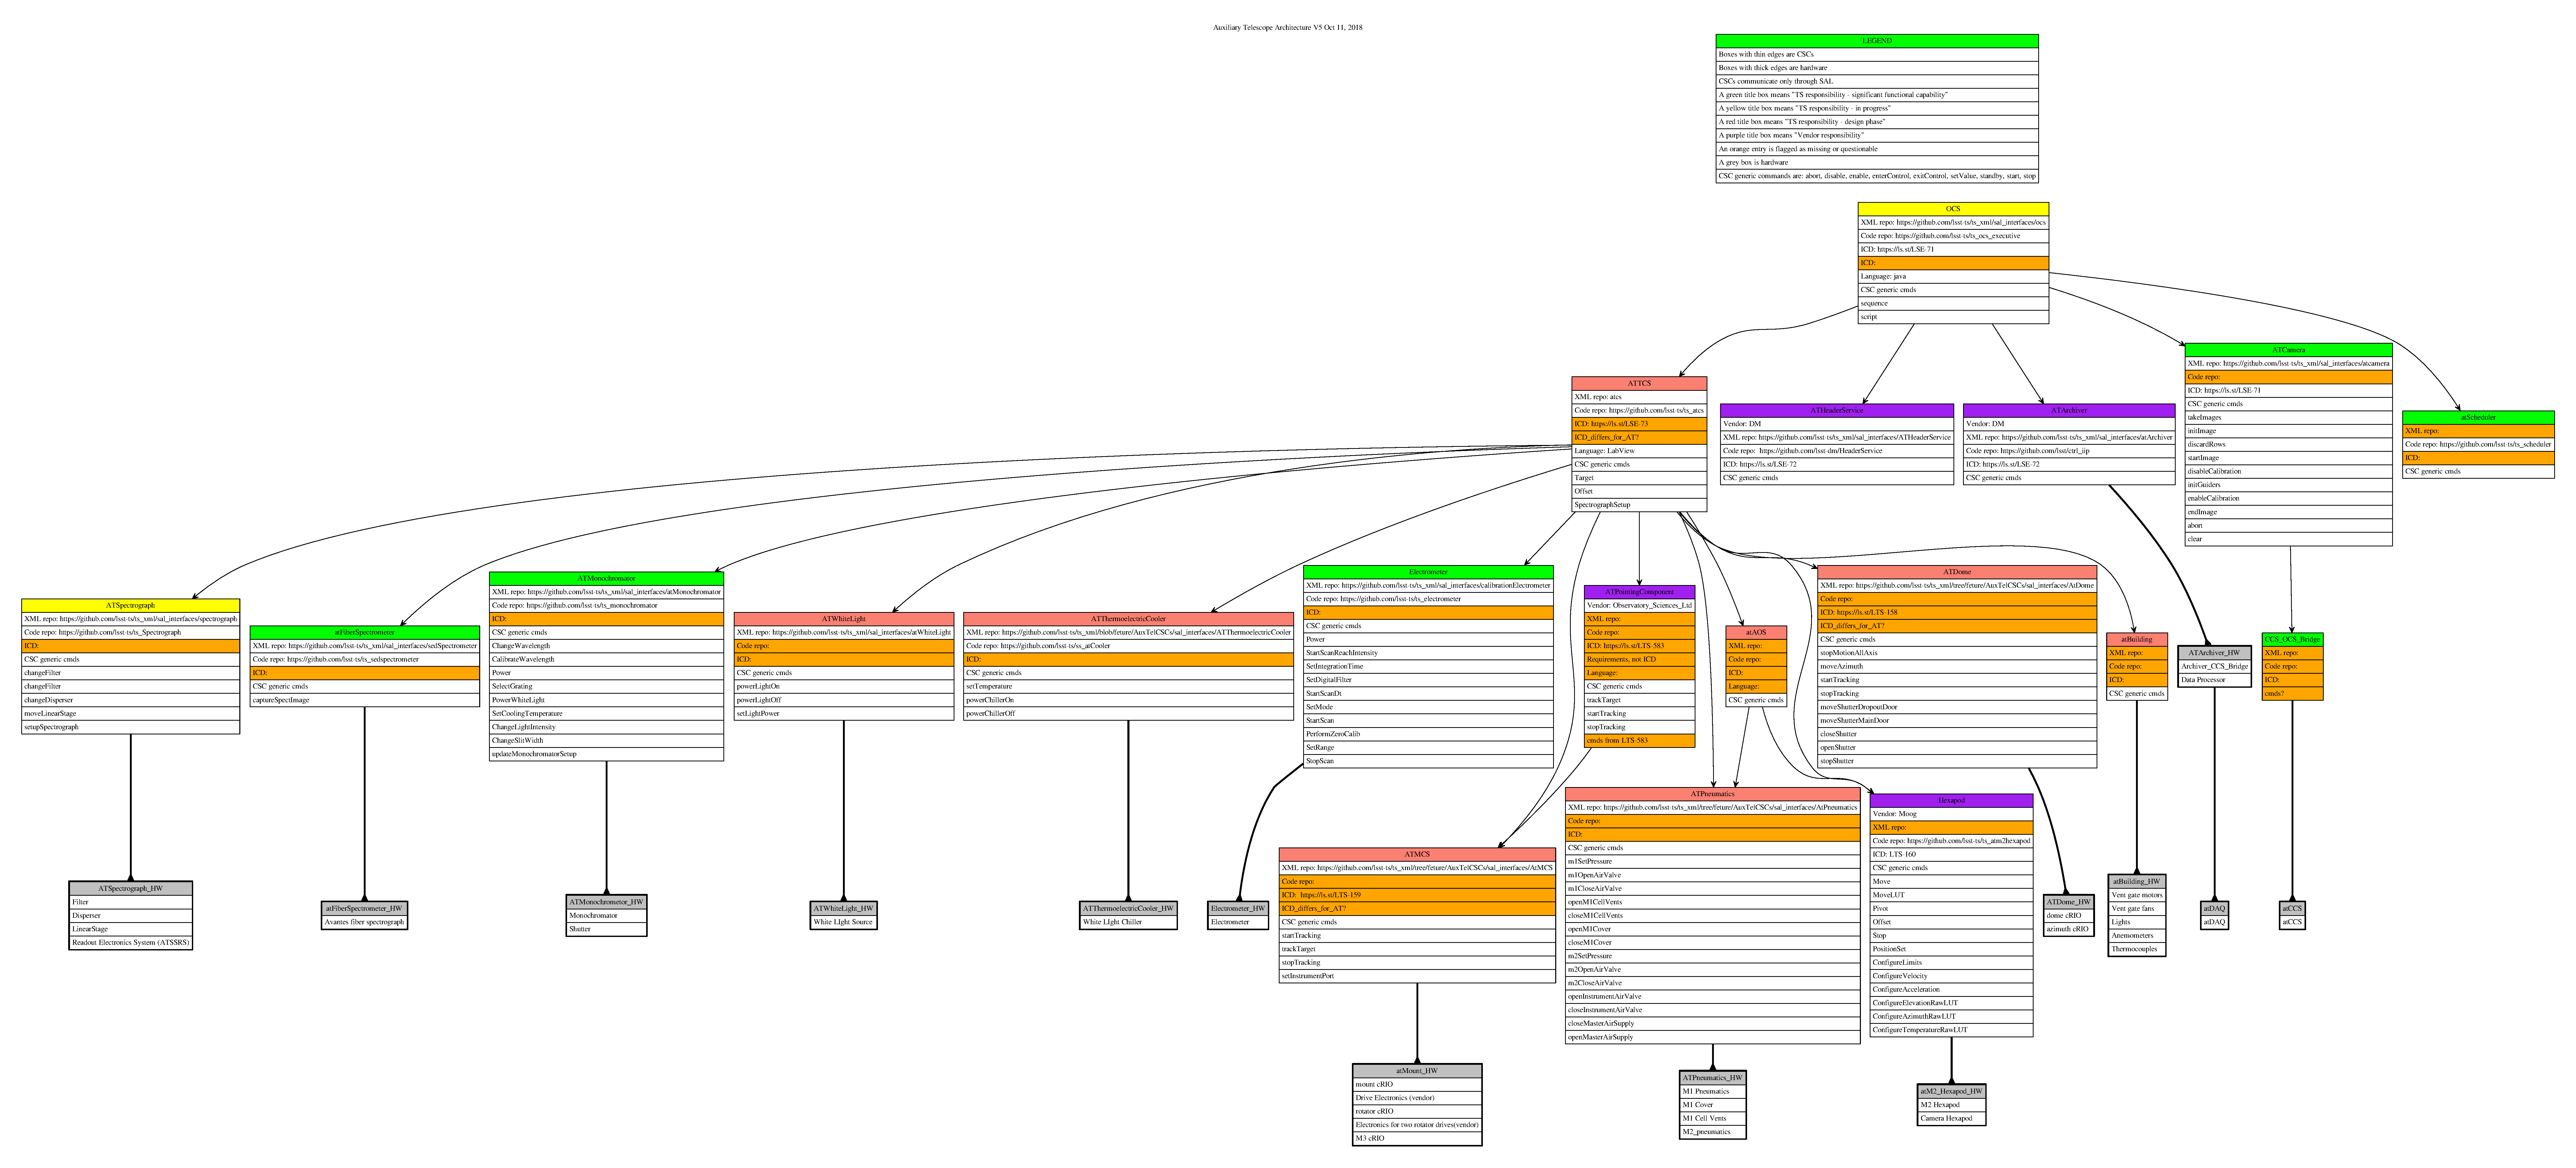
\includegraphics[width=0.9\textwidth]{AT}
\caption{Complete set of AT CSCs (preliminary)\label{fig:atcscs}}
\end{center}
\end{figure}

\begin{figure}
\begin{center}
\includegraphics[width=0.9\textwidth]{LSST}
\caption{Complete set of MT CSCs (preliminary)\label{fig:mtcscs}}
\end{center}
\end{figure}

\subsection{SalObj - Python and scripting }\label{sect:salobj}
SalObj is a Python library provides a pythonic and object-oriented interface to create CSCs and SAL Scripts that can be executed by the script queue component (see Sect.~\ref{sect:scriptq}). The library defines two sets of base classes that are mirror to each other, Remote and Controller. A Remote will send commands to and receive telemetry and events from a specific component whereas a Controller will receive commands and publish telemetry and events. In this framework, a CSC is a specialized Controller that is configured to perform some basic actions by default. %A high level diagram is provided in \figref{fig:salobj}.

Internally, SalObj uses the python library \asyncio\footnote{\url{https://docs.python.org/3/library/asyncio.html}} to handle the inherently asynchronous nature of the SAL messaging system.

% \begin{figure}
% \begin{center}
% 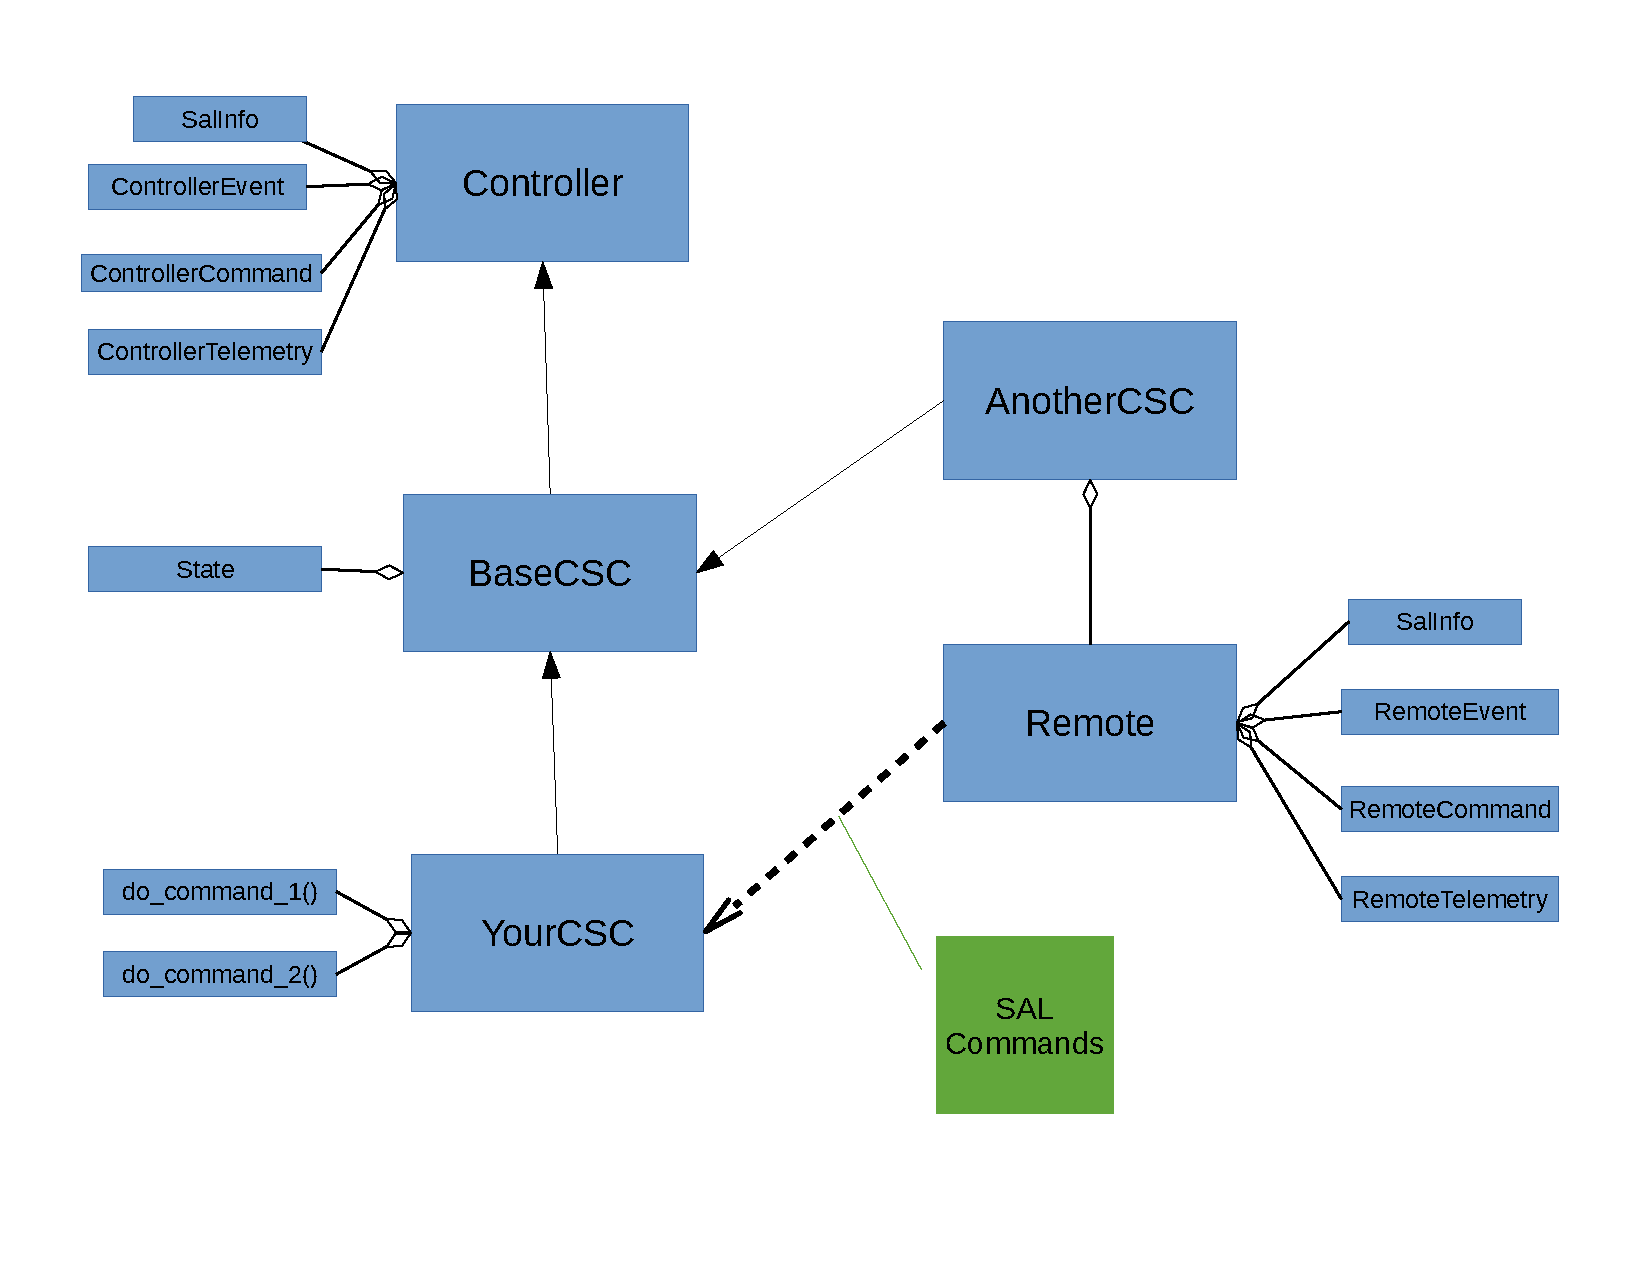
\includegraphics[width=0.9\textwidth]{SalobjClassDiag2}
% \caption{SalObj python scheme for  CSCs\label{fig:salobj}}
% \end{center}
% \end{figure}

\subsection{Hardware interface components}\label{sect:hardware_csc}
Probably the most critical or sensitive components of the LSST system architecture are those that directly control hardware. Some of these components are going to be delivered directly by external vendors, such as those that will control the main telescope mount (MTMount) and the main telescope secondary mirror (MTM2). There are also those that are developed in house, e.g. the main telescope M1M3 (MTM1M3).

In some special cases, where fast real time response is required, it is highly desirable that the control software and hardware are part of an integrated system. For those systems, the components are developed either using the LabView component template, which is part of the LSST infrastructure or in C++ developed using the low level SAL API.

In most other cases, the hardware comes with a control software that can be easily interfaced by using standard protocols (such as TCP/IP or serial ports), and there is no special need for the component software to reside close to the low level hardware controller. In those cases, the components are written in Python using the SalObj library which is also part of the LSST infrastructure. By writing these components using a unified language and library (Python+SalObj) we allow a high level of flexibility and maintainability of the software and considerably decrease the development cycle.

\subsection{Pure software components}\label{sect:software_csc}
In the LSST System Architecture there are a number of components that, even though they do not control hardware directly, dictate what hardware components are supposed to do. Some of these components are responsible for heavy computational routines, such as the Optical Feedback Control (MTOFC), which is responsible for applying corrections to both M1M3, M2 and hexapod components for the main telescope or even the Scheduler, which is responsible for processing an entire set of observatory telemetry information and history of observations to compute an observing queue.

These pure software components are mostly written in Python using SalObj library. There are three special cases of these components that form the basis of the LSST System Architecture; the ScriptQueue (Sect.~\ref{sect:scriptq}), Control Systems (Sect.~\ref{sect:ocs}) and the Watcher (Sect.~\ref{sect:watcher}). Together, they provide the tools needed for integration, commissioning and operation of the observatory.

\subsection{Configuration Management}\label{sect:config}
During commissioning and operations, LSST will have a large number of running software components under the purview of DM, Camera, and TSS. In general, the behavior of each of these components is modifiable through configuration information which is read in during startup of the component, or possibly changed while the component is running. Careful management of this configuration information is crucial to reliable functioning of the Observatory, and to the analysis of its data products.

In this context, git is the solution adopted to store and manage different sets of configurations and different versions of configurations. Git is already a standard in industry as a software management tool and has becoming increasingly used to manage general documents and files as well, not to mention that it is already readily available and broadly adopted by the project. {\color{blue} Therefore, each component must establish a {\bf separate} git repository to store its configuration files.

These configuration repositories will be hosted on a configuration server at the summit so that, even if communication with the base or the internet is not available, components still maintain access to their configuration repositories. Different configuration sets (or labels) are stored in separate branches, and tags can be created to specify immutable sets.

Several options for configuration file format, and their associated software tools, have been considered. Each of the available options naturally has its strengths and weaknesses, and none stand out as being particularly useful for all LSST use cases (and/or available for all the project adopted programming languages).

For components written in Python, \pexC~is the adopted solution. As an overview of \pexC, here are a few snippets from the library documentation:

\begin{quotation}
The \texttt{lsst.pex.config} module provides a configuration system for the LSST Science Pipelines.... Configurations are hierarchical trees of parameters used to control the execution of code.... Configurations are stored in instances of a "config" object, which are subclasses of the \texttt{Config} class. Different configuration sets are associated with different subclasses of \texttt{Config}. For example, in the task framework each task is associated with a specific \texttt{Config} subclass.... Configuration objects have \texttt{fields} that are discrete settings. These \texttt{fields} are attributes on config classes.
\end{quotation}

In the TSS context the "task" above becomes a "CSC".

\texttt{lsst.pex.config.Config} class has methods \texttt{save()} and \texttt{load()} which persist and restore class instances from files, which just contain Python code. Note that because these files are Python code, it is easy to include documentation within the files.

The validation of a \texttt{Config} file is handled by the \texttt{\_\_init\_\_()} method of the \texttt{Config} subclass which can check, for example, whether parameter values comply with range limits, or whether all required parameters are specified.

In this framework, the configuration schema (or definition) will be developed and stored in the CSC codebase repository (using \pexC). As already stated above, a separate repository hosts the actual configuration files which, in the case of \pexC, only contains changes to the default set of values.}

%The use of git in required to maintain history and recoverability of the changes to default configuration values and fulfill the requirements for a Configuration Management system for LSST.

%Nevertheless, since \texttt{pex\_config} is a Python library, it is not readily available for other languages used throughout the system. In order to overcome that issue, we provide a Configuration Adaptor that components written in other languages can connect through a regular TCP/IP connection.

%

%For CSCs that a not developed in Python, the Configuration Adaptor will be responsible for reading the \texttt{pex\_config} configuration definition and also











